\section{Übung 13}
\begin{minipage}[t]{0.33\textwidth}
	$\underline{\text{Gegeben:}}$
	\begin{itemize}
		\item $H = \SI{3}{\meter}$
		\item $R = \SI{200}{\milli \meter} = \SI{0,2}{\meter}$
		\item $T_{\ce{H2O}}= \SI{20}{\celsius}$
	\end{itemize}
\end{minipage}
\begin{minipage}[t]{0.33\textwidth}
	$\underline{\text{Gesucht:}}$
	\begin{itemize}
		\item $\overrightarrow{F}_{\text{res}}$
	\end{itemize}
\end{minipage}
\begin{minipage}[t]{0.33\textwidth}
	$\underline{\text{Verwendete Formeln:}}$
		\begin{equation}
			p = \rho*g*h
		\end{equation}
		\begin{align}
			\overrightarrow{F} &= A*p \\
			&= \rho*g*V
		\end{align}
		\begin{equation}
			A = \pi * r^2
			\end{equation}
\end{minipage}

\textit{Zur Erinnerung: }
\begin{flalign*}
	\left[ \si{\kg \per \kmeter}*\si{\per\raiseto{2} \second} = \si{\newton \per \smeter} = \si{\pascal}\right]\\
\end{flalign*}

\begin{flalign}
	\text{\textbf{Annahme}: Da } T_{\ce{H2O} }= \SI{20}{\celsius} \text{ ist, ist } \rho_{\ce{H2O}} = \SI{1000}{\kg \per \kmeter}
\end{flalign}

\begin{figure}[h!]
	\centering
	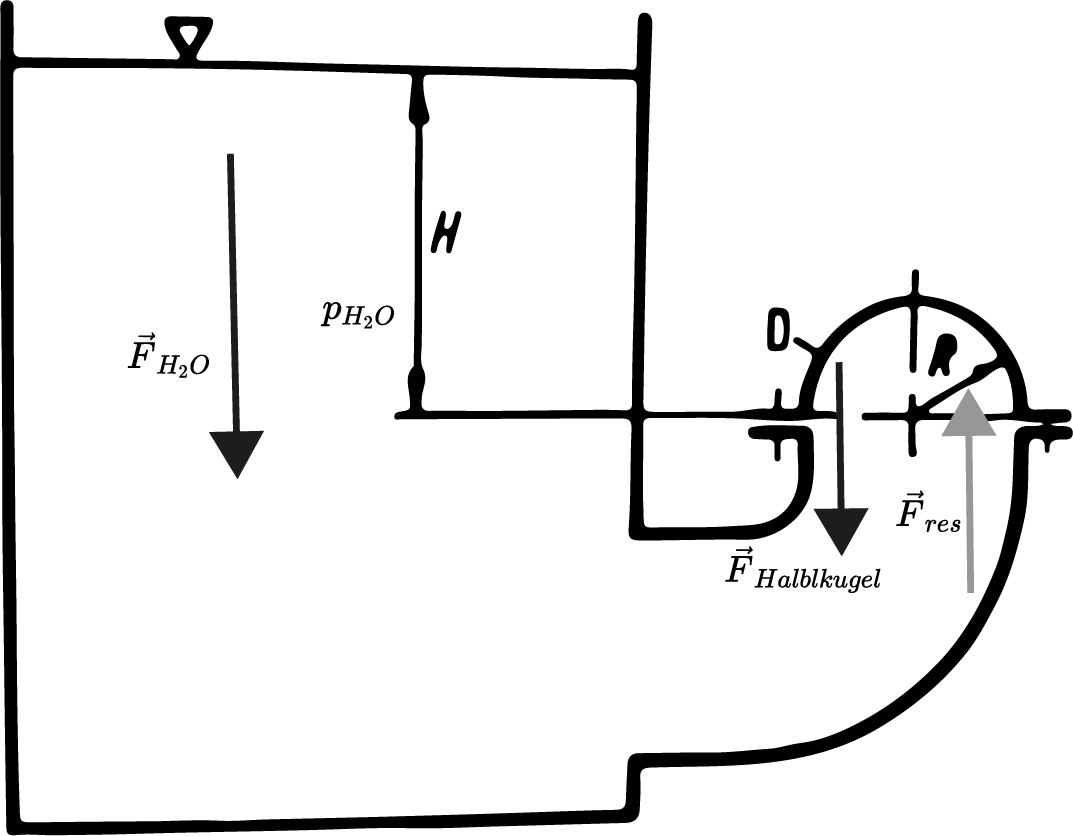
\includegraphics[width=0.4\textwidth]{u13}
\end{figure}
\FloatBarrier
%Ende

\begin{flalign}
	p_{\ce{H2O}} &= \rho_{\ce{H2O}}*g*h\\
								&= \SI{1000}{\kg \per \kmeter}*\SI{9,81}{\meter \per \raiseto{2} \second}*\SI{3}{\meter}\\
								&= \underline{\SI{29430}{\pascal}}
\end{flalign}
\begin{flalign}
	A_{\text{Halbkugel}} &= R^2*\pi\\
	&= \SI{0,2}{\meter}^2*\pi\\
	&= \underline{\SI{0,126}{\smeter}}
\end{flalign}
\begin{flalign}
	\overrightarrow{F}_{\text{\ce{H2O}}} &=A_{\text{Halblkugel}}*p_{\ce{H2O}}\\
	&= \SI{0,126}{\smeter}*\SI{29430}{\newton \per \smeter}\\
	&= \underline{\SI{3698,3}{\newton}}
\end{flalign}
\begin{flalign}
	\overrightarrow{F}_{\text{Halblkugel}} &=\rho_{\ce{H2O}}*g*V_{\text{Halbkugel}}\\
		&= \SI{1000}{\kg\per\kmeter}*\SI{9,81}{\meter \per \raiseto{2}\second}*\frac{1}{2}*\frac{4}{3}*\pi*\SI{0,2}{\smeter}^3\\
		&= \underline{\SI{164,4}{\newton}}
\end{flalign}
\begin{flalign}
	\overrightarrow{F}_{\text{res}} &=\overrightarrow{F}_{\ce{H2O}}-\overrightarrow{F}_{\text{Halblkugel}} \\
			&= \SI{3698,3}{\newton}-\SI{164,4}{\newton}\\
			&= \underline{\underline{\SI{3533,9}{\newton}}}
\end{flalign}
